\chapter{The role of science communication}
This chapters presents a very concise overview of the importance of science communication in modern society. Section \ref{The_knowledge_era} outlines the characteristics of the knowledge era. Section \ref{Challenges_in_the_knowledge_era} focuses on the economical and societal challenges rising in the knowledge era. Section \ref{The_scientific_citizenship} highlights the importance of scientific citizenship. Section \ref{The_scientific_citizenship} considers the need for science communication to let individuals acquire the scientific citizenship. 

\section{The knowledge era} \label{The_knowledge_era}
Three economical eras have been identified in the history of human civilisation \cite{Aasi1}. The first one was the agricultural age. This is believed to have started between 10000 and 8000 B.C. in different regions in the world. The second era is the industrial one. It began in England in the 18th century as a result of the industrial revolution. The third era is the knowledge age, and it is the one into which human civilization is currently entering. 

The three eras are based on different primary production resources. For the agricultural age, these were the work of people and animals. In the case of industry-driven economy, the ultimate source of richness and development is the work of people and machines. On the contrary, the knowledge era is not founded on the capacity to produce and accumulate tangible goods, but rather on the ability to store, generate and apply new information.

The information on which the knowledge age is based is mainly scientific. In the past centuries, the impact of science on humanity has been growing without interruption. Nowadays, the outcomes of scientific activities permeate our society and heavily shape our life style. Examples range from telecommunications to cancer cures, or from artificial intelligence to the development of new materials.

The reason for the increasing impact of science is the peculiar nature of knowledge as a resource. Just like any other resource, it is important for its capacity to provide solutions to problems. However, contrarily to resources such as water, gold or oil, scientific knowledge is potentially unlimited, as it is capable of generating itself (knowledge leads to new knowledge). Moreover, the same knowledge can be used simultaneously by multiple entities. Hence, scientific knowledge is intrinsically a non-exclusive good.

For its characteristics as a resource, scientific knowledge has revolutionised the economy on a planetary level. The ongoing, science-driven change of the global market has introduced countless positive innovations. However, it has also lead to dramatic societal changes.   

\section{Challenges in the knowledge era} \label{Challenges_in_the_knowledge_era}
The relationship between scientific research and society has changed significantly after the second world war. From the half of the past century, several countries have started using science and its generation of new knowledge and technology as a source of economical growth. This process has progressively become more intense over the past decades. Nowadays, the national economies showing the highest growth rates are those of countries investing significant fraction of their gross domestic product in research and development. Examples are the United States, Northern Europe and Asiatic countries such as China, India and South Korea.   

\begin{figure}[!t] 
 \begin{center}
 %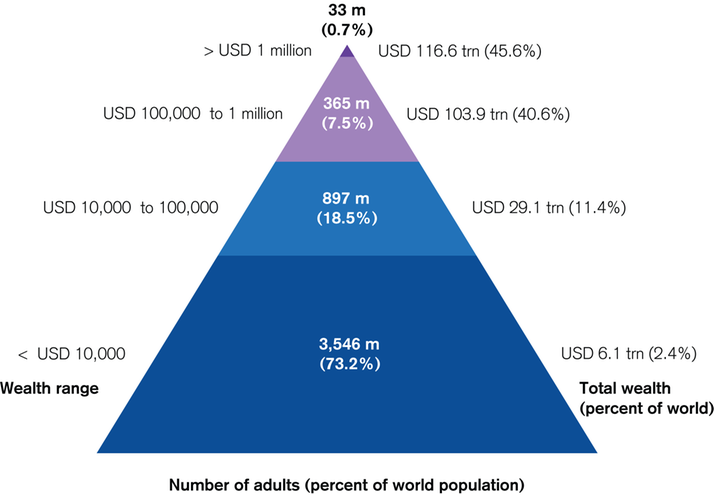
\includegraphics[width = 8.0 cm, height = 6.0 cm]{Images/Global_wealth_pyramid.png}
 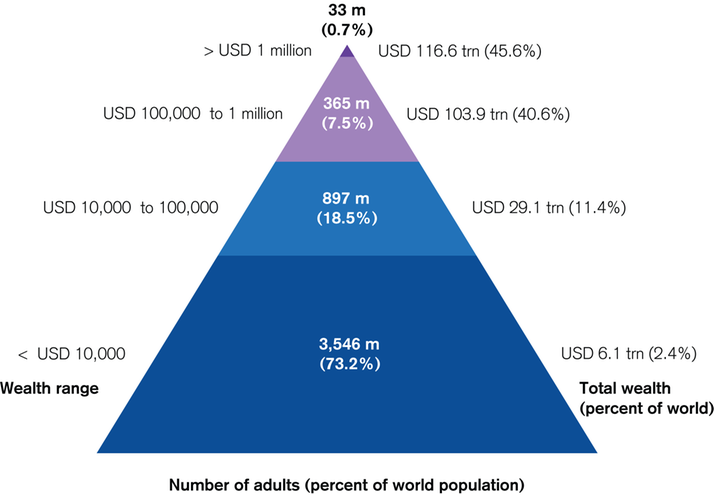
\includegraphics[scale=0.3]{Images/Global_wealth_pyramid.png}
 \caption{Graphic representation of the $M - \sigma$ relation. Observations suggest a correlation between the mass of the putative SMBHs hosted in the galactic centers and the velocity dispersion $\sigma$ of the galaxy. Original image in.}
 \label{M_sigma_relation}
 \end{center}
\end{figure}

The capacity of scientific knowledge to generate richness has attracted a growing number of private investors. As a result, in many countries private investments on scientific research are larger than public funds. One example are the United States, where private funding is twice as large as the public one. 

\begin{figure}[!t] 
 \begin{center}
 %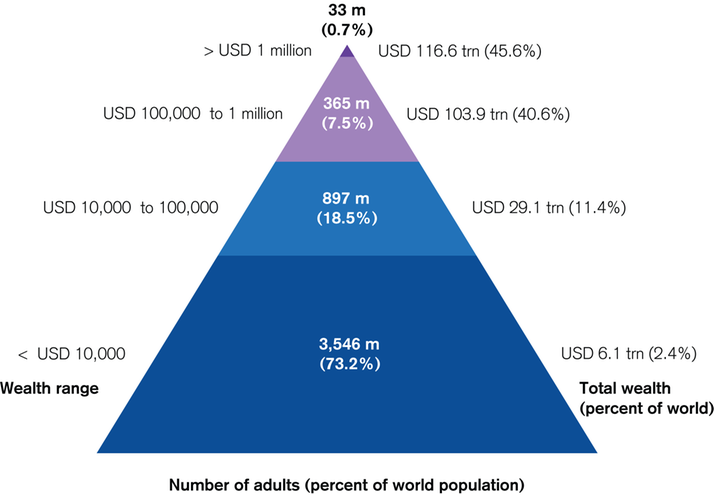
\includegraphics[width = 8.0 cm, height = 6.0 cm]{Images/Global_wealth_pyramid.png}
 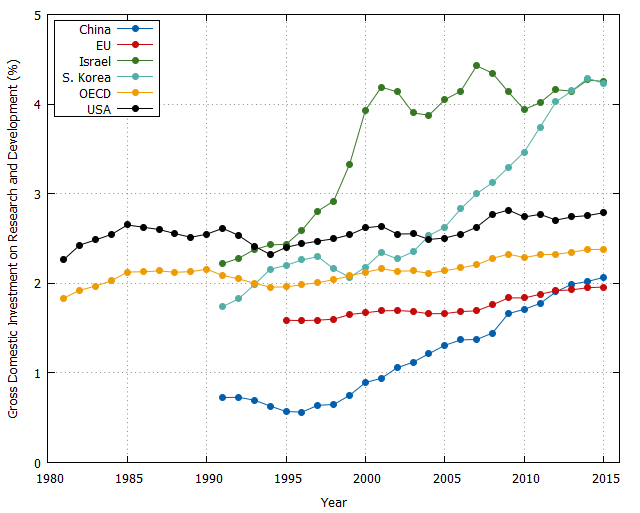
\includegraphics[scale=0.3]{Images/GD_investment.png}
 \caption{Graphic representation of the $M - \sigma$ relation. Observations suggest a correlation between the mass of the putative SMBHs hosted in the galactic centers and the velocity dispersion $\sigma$ of the galaxy. Original image in.}
 \label{M_sigma_relation}
 \end{center}
\end{figure}

The leading role of private investors is based on a reinterpretation of knowledge as a resource. To pursue personal profit, investors are typically non interested in sharing the knowledge they have developed or they way they have used it to create goods. This approach limits the possibility to generate new knowledge from the results of others. Moreover, those with limited buying power cannot afford specific classes of products and hence cannot benefit from the knowledge behind them. One example are patented expensive medicines. In such a scenario, knowledge as a resource partially looses the intrinsic characteristics of being unlimited and non exclusive mentioned in Section \ref{The_knowledge_era}. 

\begin{figure}[!t] 
 \begin{center}
 %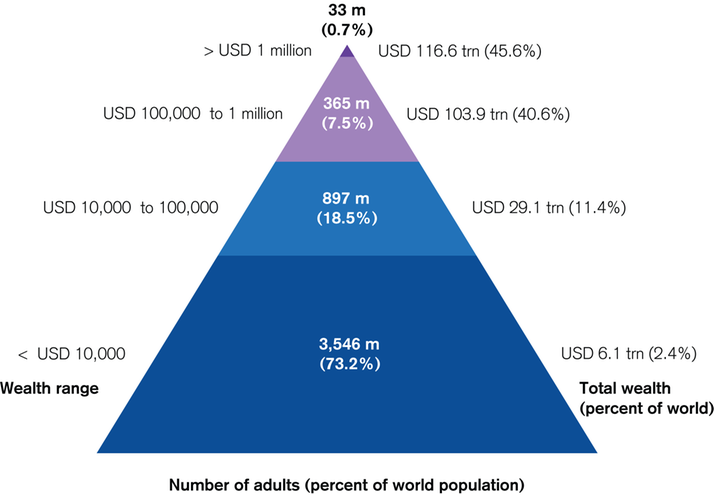
\includegraphics[width = 8.0 cm, height = 6.0 cm]{Images/Global_wealth_pyramid.png}
 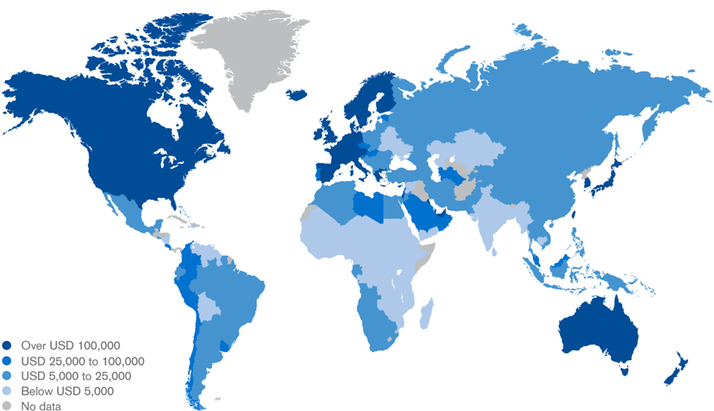
\includegraphics[scale=0.3]{Images/World_wealth_levels.png}
 \caption{Graphic representation of the $M - \sigma$ relation. Observations suggest a correlation between the mass of the putative SMBHs hosted in the galactic centers and the velocity dispersion $\sigma$ of the galaxy. Original image in.}
 \label{M_sigma_relation}
 \end{center}
\end{figure}

The current knowledge-driven development of the global economy has two important consequences. Firstly, humanity is richer than ever before. Secondly, the progressive concentration of the generated richness in the hands of few individuals is causing societal inequality. 

The increasing inequality is an obstacle for the creation of a democratic society. The scenario humanity is facing can be changed if knowledge will not be used as a mere instrument of power, but rather as a common good everyone should benefit from. This paradigm shift is one of main goals of the scientific citizenship.

\section{The scientific citizenship} \label{The_scientific_citizenship}
The potential of scientific knowledge to become a pillar of democratic societies was first recognised by the English philosopher Francis Bacon in the 17th century. He proposed that science and technology should not bring advantages to a limited number of societal groups or nations, but rather to the whole humankind. This vision is efficaciously outlined in his utopian novel New Atlantis.

Bacon's ideas are extremely topical. As mentioned in Section \ref{Challenges_in_the_knowledge_era}, the access to the goods generated by scientific research is fundamental to prevent societal divisions and exclusions.

A second ingredient for the creation of a democratic society is the people's awareness of the scientific process, as well as of its goals, outcomes and limits. In fact, a democratic society is funded on the participation of citizens when decisions impacting the community must be taken. Because of the permeating role played by science in today's society, science-related issues are no exception. Examples are topics such as mandatory vaccination, euthanasia, abortion, animal experimentation, alternative medicine, nuclear energy, recycling and, in general, the investments on research assigned by policy makers. Hence, a better understanding of science \textit{modus operandi} is a key factor to ensure effective participatory processes.    

The population's engagement in the decision-making process is fruitful if scientific innovations are neither passively accepted nor irrationally feared. To this aim, people must be given the ability to intervene in an informed, rational and critical way. This scenario is only possible if individuals are formed and trained in an adequate cultural context. In other words, if people acquire the so-called scientific citizenship.

How to best prepare individuals to become scientific citizens is still debated. Nevertheless, a key ingredient has been identified in the need to bring scientists and citizens closer to each other. It is widely accepted that the construction of a democratic knowledge era depends crucially on the continuous dialogue and information and knowledge exchange between these two communities. A paradigm explaining the growing importance of science communication.

\section{Science communication and modern society}    
Science relies heavily on communication. To be useful, research results must be communicated to the rest of the scientific community. This has became even more crucial in the era of Big Science. Modern physics offers illustrative examples in this direction. Large-scale experiments such as the LHC particle accelerator at CERN in Switzerland or the LIGO-Virgo gravitational-wave observatories in the USA and Italy are built and maintained by international collaborations of thousands of scientists from tens of different countries. These titanic efforts can only be successful if supported by effective internal communication.  

The relationship between science and communication has evolved with the transition to the knowledge era. Nowadays, science communication can no longer happen exclusively within the scientific community. As outlined in Section \ref{The_scientific_citizenship}, the construction of a democratic society requires the engagement of disparate societal groups in the decision-making processes related to scientific questions, such as scientists, policy makers, private investors, non-governmental organizations, citizens etc. Hence, when discussing with each other these groups make science communication.

The disparate societal groups have different cultural background and objectives. Thus, they adopt different languages when talking about scientific issues. Moreover, science communication is most effective when properly tuned on the targeted audience. The optimal choice depends on both the content and the choice of the considered communication channel. As a consequence, numerous different kinds of science communication exist.   

The present thesis focuses on the science communication aiming to inform citizens on a non-technical level of current investigation lines. This is the oldest type of communication science external to the scientific community. The first example in this direction was the \textit{De Rerum Natura} by the Roman poet Lucretius in the first century BC. Another historically very important book was Galileo Galiei's \textit{Sidereus Nuncius} in the XVII century. The work rapidly spread all over the world short after its publication and propagated the author's astronomical discoveries.

More specifically, this thesis focuses on a specific class of EU-funded research project and on their use of the web 2.0 social media to communicate their results and objectives. As outlined in the next chapters, the ultimate goal is to investigate whether European scientists are properly exploiting today's most effective communication channels to inform citizens about two of the future's most important scientific challenges: the development of quantum technologies and supercomputers.

\section{Chapter summary} 
In this chapter, the following items have been discussed:

\begin{enumerate}
 \item Human society is currently entering into the so-called knowledge era. This age is characterised by the fact that scientific knowledge has become one of the most important sources of wealth. 
 \item The knowledge era offers unprecedented opportunities to improve people's life quality. However, it also present new challenges to human society. In particular, the unequal access to scientific knowledge and technology may prevent the realisation of democratic systems.
 \item The construction of a democratic society in the knowledge era depends also on the active engagement of citizens and stakeholders in the debate on the impact of scientific issues on their lives. This can be achieved if people are trained to discuss about scientific questions in a constructive and critic way, i.e., if individuals acquire the so-called scientific citizenship.
 \item One key factor to let people acquire the scientific citizenship is science communication. There exist disparate kinds of science communication, depending on the interacting societal groups. The present thesis focuses on science communication adopted to inform citizens via social media of recent developments in European research projects.     
\end{enumerate}